\documentclass{article}
\usepackage[utf8]{inputenc}
\usepackage[a4paper, margin=2.5cm]{geometry}
\usepackage{graphicx}
\usepackage[french]{babel}

\usepackage[default,scale=0.95]{opensans}
\usepackage[T1]{fontenc}
\usepackage{subfig}

% pour les hyperlien 
\usepackage{hyperref}
\hypersetup{
    colorlinks=true,
    linkcolor=blue,
    filecolor=magenta,      
    urlcolor=cyan,
    pdftitle={Overleaf Example},
}
\urlstyle{same} % utiliser \href{url}{Text}

\title{Les interactions fréquentes chez les plus jeunes avec des systèmes de dialogues ont-elles baissé leurs attentes face à ces systèmes ?}
\author{Charles Vin}
\date{Décembre 2021}

\begin{document}
\maketitle \newpage

\section{Introduction}
Lors d'un dialogue oral, pour un partage d'information efficace en terme de temps et de compréhension, chaque interlocuteur doit prendre en compte les connaissances de l'autre et s'adapter à celui-ci \cite{clark_1996}\cite{TunerKnutsen}. En effet, si ce n'est pas le cas, les conversations pourraient être trop détaillées et donc longues, ou alors à l'opposé, trop précises et donc complexes pour la compréhension de l'autre. Ainsi, les participants vont implicitement s'accorder sur le sens des termes employés en utilisant des indices linguistiques et physiques de l'environnement \cite{Clark1981-CLADKA}. Cette connaissance implicite fait référence au terrain commun, définie par l'ensemble des connaissances que deux « entités » partagent et ont conscience de partager \cite{clark_1996}\cite{Clark1981-CLADKA}\cite{stalnaker1978a}.

Pour mesurer ce phénomène, on utilise le très connu paradigme de Clark et Wilkes-Gibbs \cite{clark1986a} où deux participants interagissent autour de figures de tangram abstraites. Chaque participant a un rôle prédéfini, l'un est appelé l'executant et l'autre le directeur. L'executant doit ordonner les figures de tangram dans un ordre prédéfini connu uniquement par le directeur. Les interactions sont libres et sans interventions de l'expérimentateur. Cette opération est répétée 6 fois avec les mêmes figures à chaque essai (uniquement l'ordre imposé varie). Typiquement, au premier essai, le directeur décrit les figures avec beaucoup de références indéfinies "la première carte ressemble a un genre de renard, mais avec une patte en moins". Au fur et à mesure des essais, les descriptions seront de plus en plus courtes avec les deux interlocuteurs s'accordant sur des références communes "Le renard amputé". L'utilisation de référence définie augmentera également avec le temps. 

% Je peux continuer de détaillé à partir de l'article de la prof 
Le terrain commun se construit par une collaboration entre les deux participants. Le premier présente une information à intégrer au terrain commun avec des indices montrant son incertitude ("un ours", "une sorte d'ours"). En retour, le deuxième va pouvoir indiquer qu'il a compris, qu'il accepte l'information présentée. Par exemple en paraphrasant ce qu'il a compris ou en disant "oui" ou "ok". Si ce n'est pas le cas, il peut le signaler à son interlocuteur qui pourra ré-expliquer. Et ce jusqu'à ce que les deux parties se soit comprises.

% Je passe sur l'intro de l'article HS
Dans les interactions humain-système, le même principe s'applique. L'utilisateur a les mêmes attentes et croyances que dans le dialogue humain-humain. Par exemple, lors d'une interaction avec un système de dialogue à propos d'objets du quotidien, l'utilisateur va réutiliser les mêmes références, les mêmes mots que le système. Assumant que celui ci doit être capable de les comprendre. 

Ces interactions avec des systèmes de dialogue sont de plus en plus fréquente de nos jours. Des assistants vocaux sont installés par défaut dans nos téléphones, des automates utilisant le langage naturel sont présents dans les gares et les aéroports pour nous permettre d'acheter des billets. Malheureusement, en attribuant les mêmes attentes que lors d'un dialogue humain, les interactions peuvent être frustrantes. En effet les systèmes sont rarement conçus pour prendre en compte les connaissances de la personne en face d'eux et construire un terrain commun. 

\subsection{Problématique}
Même si l'utilisation de ces systèmes tend à se démocratiser pour tous et notamment dans l'aide à la personne. On peut supposer que les moins âgés d'entre nous en ont une utilisation plus fréquente que les plus âgés. Ils ont ainsi fait face à de plus nombreuses déceptions face à ces systèmes que des personnes âgées. Dans cette étude, nous allons examiner l'idée que cette frustration a diminué les attentes en terme de dialogue et d'utilisation du terrain commun chez les jeunes lors des interactions humain-système. 

Pour cela, nous avons utilisé le paradigme de Clark et Wilkes-Gibbs décrit plus haut, lors d'une interaction avec un système de dialogue factice, en faisant varier l'âge des participants et le design du robot. En effet, les indices présents dans l'environnement peuvent agir sur les suppositions faites à propos des connaissances communes \cite{PowersRobot}. Faire varier ce paramètre aux deux extrêmes permet d'obtenir de plus gros effets dans les résultats tout en contrôlant son possible effet parasite (l'utilisateur a associé la frustration uniquement avec un certain type de système).

\subsection{Hypothèses} \hypertarget{HP}{} % emplacement de cette section
En faisant varier l'âge, les plus jeunes étant habitués aux systèmes de dialogue de la vie quotidienne ne s'adaptant pas ou très mal à leur interlocuteur. On peut s'attendre à ce qu'ils construisent un terrain commun plus lentement que des personnes plus âgées.

En faisant varier le type d'agent, on peut penser que face à un robot humanoïde avec une modalité orale, les participants aient plus tendance à présupposer un terrain commun et donc à le construire plus rapidement.

On peut également s'attendre à une corrélation négative entre la fréquence d'utilisation des systèmes de dialogue et la vitesse d'installation d'un terrain commun.


\section{Méthode}
Nous avons donc adapté le paradigme de Clark et Wilkes-Gibbs dans le cadre d'une interaction humain-système. Comme nous étudions uniquement l'aspect interaction et communication dans le dialogue, le robot n'a pas besoin d'être doté d'une intelligence. Ce sera ici un expérimentateur qui répondra et interagira avec le participant à son insu, à la manière du magicien d'Oz. L'important est que le sujet pense qu'il interagit avec une machine.

Pour cette expérience, le robot joue le rôle de l'executant, il doit retrouver les cartes pour les remettre dans l'ordre. Et ce à partir de la description faite par le participant, qui lui, joue donc le rôle de directeur. Le robot est tout à fait capable de poser des questions et de répondre à celles du sujet. L'échange est très naturel en dehors du délais de réponse du robot d'environ 3 secondes. \\
Traditionnellement, les deux sujets vérifient leurs réponses à la fin de l'essais. Ici une fois la carte devinée par le robot, celui-ci peut l'afficher dans l'écran de la salle d'expérimentation et en débattre avec le participant. Il y a 6 cartes par essai et 6 essais.

\subsection{Plan expérimental}
En faisant varier l'âge et le type d'agent, nous sommes donc face à un plan carré latin avec 2x2 conditions  :
\begin{itemize}
    \item Âge des participants : \begin{itemize}
        \item Groupe 20 (G20)
        \item Groupe 50 (G50)
    \end{itemize}
    \item Type d'agent :\begin{itemize}
        \item Humanoïde
        \item Non-Humanoïde
    \end{itemize}
\end{itemize}

Pour mesurer la construction du terrain commun, les dialogues seront enregistrés, transcrit. Les variables suivantes seront extraites pour caractériser le dialogue :
\begin{itemize}
    \item Nombre de mot produit en moyenne par essais
    \item Probabilité d'utiliser un mot Hedge
    \item Probabilité d'utiliser des références définies
\end{itemize}

Finalement, un questionnaire permettra de mesurer le taux d'interaction quotidienne avec des systèmes de dialogue de chaque participants. Ce score permettra une analyse intra-participants avec le calcul d'un coefficient de corrélation. (Voir \hyperlink{questionnaire}{Annexe}).

\subsection{Participant}
Nous avons recruté $ n $ participants qui ont tous pour langue maternelle le français.

Pour le premier groupe (G20), les participants auront une moyenne d'âge de 20 ans avec un nombre d'hommes et femmes équilibré, typiquement des étudiants.

Pour le deuxième groupe (G50), les participants auront une moyenne d'âge de 50 ans avec un nombre d'hommes et femmes équilibré.

\subsection{Matériel}
Six images de tangram ont été choisies puis placées aléatoirement sur une grille de six colonnes et six lignes. Les cases de chaque ligne étaient numérotées de un à six. Cette grille fût imprimée. Le sens d'utilisation de la feuille était indiqué par une phrase qui rappelait la consigne dites à l'oral. Pour des exemples d'images de tangram se référer à la figure \ref{tangram}.

\begin{figure}[!htbp]
    \centering
    \includegraphics*[width=.75\textwidth]{./tangram.png}
    \caption{Exemple de figure de tangram utilisé par les participants}
    \label{tangram}
\end{figure}

Quant aux robots, notre choix s'est porté sur Nao de SoftBank Robotics. Très utilisé dans le milieu de la recherche et de l'éducation, il est peu cher et facile à programmer. Il sera utilisé dans la condition humanoïde avec ces animations et émotions par défaut. Dans l'autre condition, nous avons utilisé un système plus proche de celui des assistants vocaux. Il prenait vie sous la forme d'une sphère animée en même temps que sa voix sur l'écran de la salle d'expérimentation. La Figure \ref{jarvis} illustre les deux robots.

\begin{figure}[!htbp]
    \centering
    \subfloat[\centering Le système de dialogue dans la condition humanoïde]{{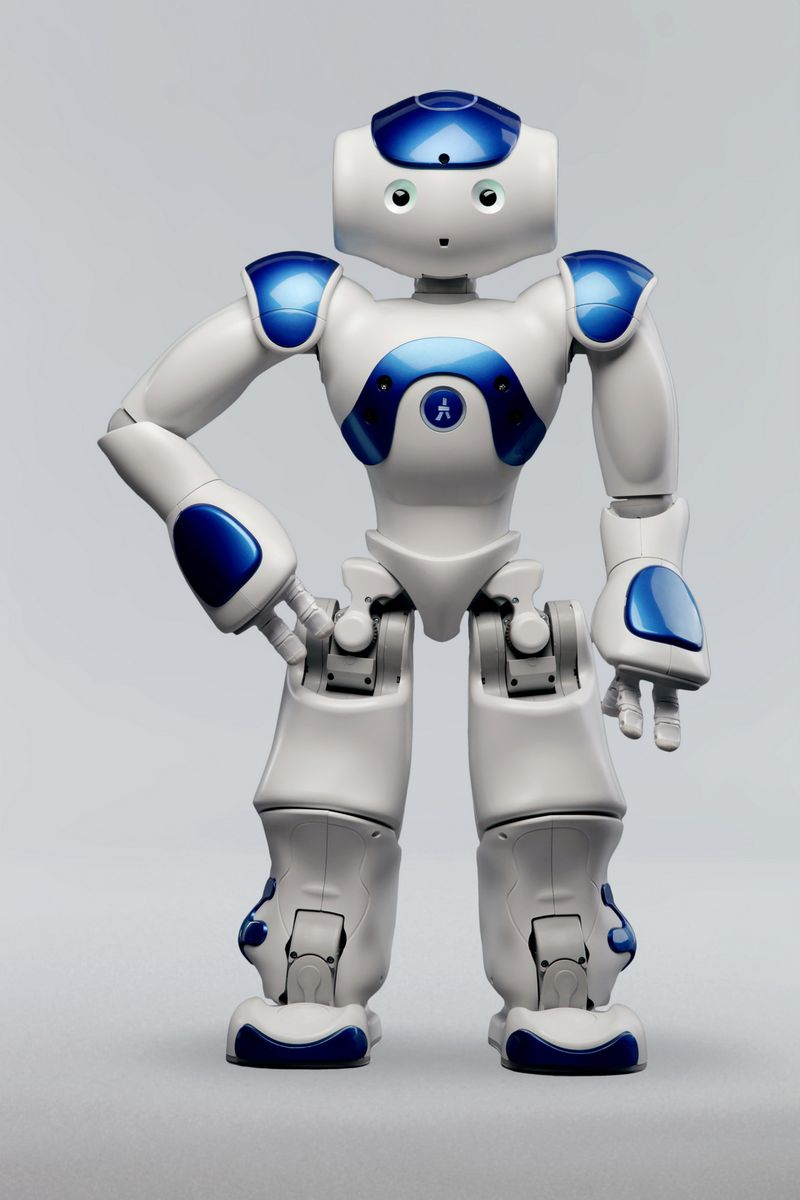
\includegraphics[width=5cm]{./Nao_robot.jpg} }}
    \qquad
    \subfloat[\centering Le système de dialogue dans la condition non humanoïde]{{
\includegraphics[width=5cm]{./gif-9.png} }}
    \caption{Les robots utilisés}
    \label{jarvis}
\end{figure}

\subsection{Procédure} \hypertarget{procedure}{}
L'expérience s'est déroulée dans une salle de passation de notre laboratoire, assis, face à un écran d'ordinateur dans la condition non humanoïde. Sinon assis face à Nao avec l'écran sur le côté droit.

Les participants avaient pour tâche de communiquer à voix haute avec le robot. Ils étaient informés qu'ils participaient à une expérience sur le dialogue humain-système et que le robot était doté d'une intelligence artificielle très performante. Mais, comme dit précédemment, en réalité derrière le robot se cachait un expérimentateur. 

La consigne pour le participant était résumé en haut de la grille de tangram mais également dites à l'oral. Il était demandé au sujet de :
\begin{itemize}
    \item Parler distinctement à voix haute
    \item De démarrer la conversation avec la description de la première image
    \item Puis de continuer naturellement la conversation avec les réponses du robot
\end{itemize}  
%ainsi que de commencer et valider sa description de l'image respectivement en commençant et en terminant par le prénom du robot et le mot clé "j'ai terminé". Après un court délais, le robot répondait en affichant sur l'écran de la salle l'image qu'il interprétait à partir de la description. Le participant pouvait ensuite répondre librement à l'interprétation du robot, toujours en commençant 

\section{Résultat attendu}
On s'attend à ce que les résultats confirment les \hyperlink{HP}{hypothèses} en suivant le paterne de la Table \ref{table1} et de la Figure \ref{graphiques}. C'est à dire que la courbe du G20 est systématiquement au dessus de celle du G50. De même pour le robot humanoïde qui faciliterait l'installation d'un terrain commun en comparaison avec le non-humanoïde. Tous ces effets seraient significatifs.

Les mesures tels que le nombre de mot par essai reflètent l'efficacité de la conversation et donc quantifient l'utilisation du terrain commun. Lorsqu'une condition utilise en moins de mot qu'une autre condition sur tous les essais, cela indique une installation plus rapide du terrain commun. Ainsi le G20 construirait plus lentement un terrain commun que le G50. On présume que cela vient de l'interaction plus fréquente avec des systèmes, éventuellement des deceptions plus fréquentes, et donc une baisse naturelle des attentes sur les capacités des systèmes à prendre en compte leur interlocuteur.

On peut penser que la forme humanoïde d'un système est un indice conditionné qui vas influencer les attentes en terme de dialogue de l'humain. Ainsi un système humanoïde provoquerait une utilisation du terrain commun plus naturelles et s'installant plus facilement. Dans nos résultats, cela se refléterait de la même manière qu'avec la condition âge.

Pour le questionnaire, on retrouverai probablement une corrélation positive entre l'utilisation des systèmes de dialogue dans la vie quotidienne et la vitesse d'installation du terrain commun. Qui appuierait l'interprétation faites dans les deux paragraphes précédant.

\begin{table}[!htbp]
    \centering
    \begin{tabular}{|l|l|l|}
        \hline
        ~ & Yougt & Old \\ \hline
        Humanoïde & - & ++ \\ \hline
        Chat Bot & - - & + \\ \hline
    \end{tabular}
    \caption{Vitesse d'installation symbolique du terrain commun en fonction des différentes conditions}
    \label{table1}
\end{table}

\begin{figure}[!htbp]
    \centering
    \subfloat[\centering Nombre de mot produit en moyenne par essais]{{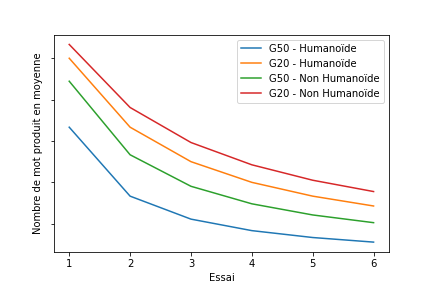
\includegraphics[width=7.5cm]{./res_attendu_nb_mot.png} }}
    \qquad
    \subfloat[\centering Probabilité d'utiliser un mot Hedge par essais]{{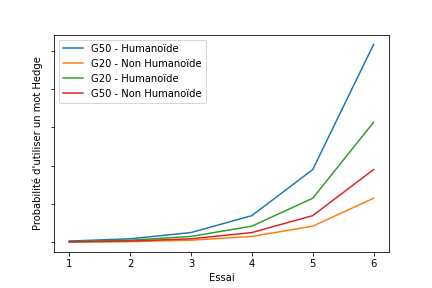
\includegraphics[width=7.5cm]{./res_attendu_hedge.png} }}
    \qquad
    \subfloat[\centering Probabilité d'utiliser des références définies par essais]{{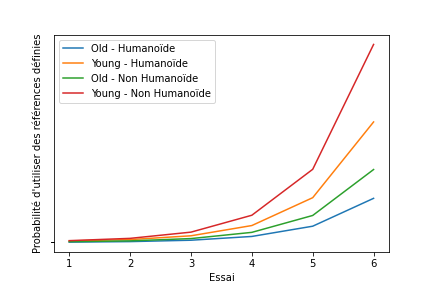
\includegraphics[width=7.5cm]{./res_attendu_ref.png} }}
    \caption{Résultats attendus}
    \label{graphiques}
\end{figure}


\section{Annexe}
\subsection{Exemple de question du questionnaire} \hypertarget{questionnaire}{}
Le questionnaire introduit la définition des termes utilisés dans les questions.
\begin{itemize}
    \item Avez-vous une enceinte connectée chez vous ? A quelle fréquence vous en servez-vous ? 
    \item Utilisez-vous l'assistant vocal de votre téléphone ? Vous a-t-il déjà frustré ou énervé ? 
    \item Les systèmes de dialogue dans les lieux publiques (gare, aéroport) vous semblent-ils utiles ? 
\end{itemize}

\bibliographystyle{unsrt}%Used BibTeX style is unsrt
\bibliography{biblio}

\end{document}